\documentclass[a4paper,twoside]{article}

\usepackage{epsfig}
\usepackage{subcaption}
\usepackage{calc}
\usepackage{amssymb}
\usepackage{amstext}
\usepackage{amsmath}
\usepackage{amsthm}
\usepackage{multicol}
\usepackage{pslatex}
\usepackage{apalike}
\usepackage{hyperref}
\usepackage{SCITEPRESS}     % Please add other packages that you may need BEFORE the SCITEPRESS.sty package.
\usepackage{hyperref}

\begin{document}

\title{Reinforcement learning methods for traffic light control: a state of the art review and TLCOPT - an open source tool for easier experimentation}

\iffalse
\author{\authorname{Ciprian Paduraru, Miruna Paduraru and Alin Stefanescu}
\affiliation{\sup{1}Department of Computer , University of Bucharest, Romania}
\affiliation{\sup{2}Department of Computing, Main University, MySecondTown, MyCountry}
\email{\{f\_author, s\_author\}@ips.xyz.edu, t\_author@dc.mu.edu}
}
\fi

\keywords{reinforcement learning, agent, traffic light control, optimization, tools, execution management.}

\abstract{Traffic light control optimization is nowadays an important part of a smart city with the advancement of sensors, IoT and edge computing capabilities. The traffic control optimization method targeted by our work follows a general trend in the community: dynamically switching traffic light phases depending on the current traffic state. Reinforcement learning was lately adopted in the literature as it has been shown to outperform previous methods. In our literature review, we found a gap in the tools that connect the research area of reinforcement learning with traffic control and simulation environments. Our primary goal in this work is to bridge this technical gap and facilitate the development of both independently. The secondary goal is to provide an introduction and overview of the state-of-the-art in reinforcement methods for the traffic signal control optimization problem. We also evaluate different algorithms for training policies to observe their performing particularities from both performance of results and efficiency.}

\onecolumn \maketitle \normalsize \setcounter{footnote}{0} \vfill

\section{\uppercase{Introduction}}
\label{sec:introduction}


A \textit{smart city} is defined by the European Commission as a place where networks and public services are efficiently harnessed through communication and information technologies for the benefit of its citizens and businesses \cite{EuropeanCommission2021}. Its aim is to create a region with sustainable economic growth and to achieve high quality in the fields of economy, mobility, environment, people, law and administration. 
The topic our group deals with is the optimization of the traffic flow within a city through an efficient management of the available traffic lights. This type of optimization is usually done by dynamically calibrating the timing of traffic signal phases at connected intersections.
As the literature review shows, the latest trend in solving this problem is through reinforcement learning (RL) methods. The main reasons for using RL methods are as follows:
(a) The optimization problem can be first simulated and optimized in a simulated environment until an optimal strategy for timing the traffic light phases is found.
(b) The current state of the art in using RL methods outperforms previous work (baseline methods), as shown in Section \ref{sec:relatedwork}.
(c) The solution chosen for intelligent traffic light control must be dynamic, making decisions over time that depend on deep insight into the overall state of the city or region being optimized.

Existing work in this area attempts to solve the optimization problem at two different levels:
\begin{enumerate}
	\item \textbf{Microscopic} - Considering the optimization of individual vehicles (e.g., how long does a vehicle wait at a traffic light), especially when optimizing a single intersection or a series of connected intersections. 
	\item \textbf{Macroscopic} - divides the physical space of the city into streets, lanes, areas and aggregates the metrics and data on large areas.
\end{enumerate}
In general, microscopic-level optimizations are more valuable and detailed, but at the cost of being harder to train and converge than macroscopic.

The purpose of the work presented in this paper is threefold:
\begin{enumerate}
	\item To provide a framework that allows separation between the methods used for optimizations and the knowledge and datasets of transportation administration. In this way, RL researchers can reuse their expertise more easily and with less technical effort to perform optimizations without knowing deep technical details about traffic management in general. On the other hand, users who are familiar with traffic management concepts can immediately reuse existing open source RL libraries out of the box with minimal knowledge in this particular area.
	\item An overview of the state of the art in reinforcement learning methods, tools, and datasets available for experimentation. This section serves as an introduction to the field for both research sides mentioned above.
	\item Comparison of state-of-the-art algorithms on a real-world dataset using the RESCO benchmark \cite{ault2021reinforcement}.
\end{enumerate}

The implementation is open source and available at \url{https://github.com/unibuc-cs/TrafficFlowOptimization}.
At the level of the framework itself, we identified the following innovations in our work:
\begin{itemize}
	\item First open source tool at the microscopic level that can leverage various modern single and multi-agent algorithms from popular open source RL libraries such as TFAgents \cite{TFAgents}, OpenAI Baselines \cite{baselines}, PFRL \cite{PFRL}, or RLlib \cite{liang2018rllib}.
	\item A comprehensive list of output options with relevant default metrics for real-world scenarios. The user can easily add new metrics around our default metrics.
	\item Code-level separation between methods used for optimization and traffic management concepts and their technical depth. See section \ref{sec:frameworkdesc} for more details.
	\item Plotting functions built on top of tensorboard, specifically adapted for the metrics of the traffic light control problem.
	\item A method to plot locations on a map and simulate traffic under various conditions, even in the absence of real-world data.
	\item Distributed training with RLlib using strategies to connect to the SUMO simulator \cite{SUMMO}. Multiple workers and/or environments per workers variants are supported.
\end{itemize}

The paper is structured as follows. Section \ref{sec:relatedwork} contains a detailed overview of RL methods used for traffic light control optimization and datasets or benchmarks available for experimentation. Section \ref{sec:frameworkdesc} contains an architectural sketch of our framework implementation and its features. Evaluation is performed in Section \ref{sec:evaluation}. Finally, conclusions and our future work plan are presented in Section \ref{sec:conclusion}.

\section{\uppercase{Related work and Introduction to the field}} \label{sec:relatedwork}

The workflow used in the literature generally consists of capturing portions of a real city with one or more intersections connected, transferring the environment and the captured real traffic data into a simulation environment, and then training algorithms to find an optimal strategy for calibrating the traffic light timing. The sub-methods used range from classical Q-learning methods to policy gradients (PG) with actor-critic to natural gradients (NG). Real-world traffic data is collected using sensors, video cameras, or statistical data on the population, its traffic patterns, lane density over time, etc. A summary of these methods can be found in \cite{SUMBA}. 

If traffic data is not available or not sufficient for a city, there are some methods in the literature that can be used to simulate and optimize strategies based on realistic data. The \textit{Four-Step} model described in \cite{ModellingTransport} and \cite{HandbookTransportModelling} is one of the most common methods to replicate real traffic flow along routes in simulated environments. The method divides the area into traffic analysis zones and then models the traffic flow considering the possible activities in the area (e.g., schools, universities, business and commercial places, etc.). Although it is used to simulate scenarios at the macroscopic level, it can also be adapted at the microscopic level by first generating probability distributions, from which the behavior is then retrieved for each individual vehicle. The \textit{Agent-Based Demand} \cite{SUMBA}, \cite{Innes2011}, traffic generation is more suited to the microscopic level by generating activities and trajectories for each vehicle agent.

We divide this section into two parts. In the first part, we present some previous work and attempts to use open-source or commercial libraries that can be used for experiments and how they compare to our work. The second part is devoted to the state of the art of algorithms used for traffic light control optimization, focusing on reinforced learning methods, which seems to be the latest trend in solving the targeted optimization problem through our work.

\subsection {Environment Simulation Tools}

The base layer of any reinforcement learning algorithm requires an environment in which it can operate. In our case study, a traffic simulator is needed that replicates real traffic data or samples from an approximately real distribution. After a review of open source tools, we concluded that SUMO \cite{SUMMO} is the most widely used and maintained tool. Users can take advantage of its ability to replay data, generate random traffic data, and it has an API to interact with from different environments, as we needed in our implementation. It also supports direct import of real parts of urban infrastructure via the OSM standard \cite{OSRM} and ASAM \cite{ASAM} (note: the difference between OSM and ASAM is that the roads in ASAM also have a 3D topology, which allows for more realistic experiments when cities do not necessarily have apartment ground). It also supports integration with CARLA \cite{dosovitskiy2017carla} for 3D simulation and visualization. An alternative to SUMO was MatSim \cite{MATSim}. However, at the moment it seems to be less maintained and provide less support than our first choice.


\subsection {Datasets}
As for datasets, we considered datasets that can either be used directly, i.e., provide data that can be used directly at the microscopic level, or that can be adapted to our goal, i.e., contain data sources that can generate probabilities that can be sampled by the simulator at simulation time. 
Caltrans \cite{Calt} collects data from street-level sensors and induction loops. It is used by the state of California to monitor traffic. The dataset, which is publicly available online, provides researchers with raw data collected from real traffic to experiment with. Induction loop data is counted and traffic density data is stored on local regional servers every 30 seconds. The dataset is created using the aggregated data from these local servers and is constantly updated. The data can be imported into SUMO simulator by connecting the locations of data sensors on longitude and latitude with the urban infrastructure obtained from OSM. A tool in our framework enables this connection in a simple way for experiments. Although originally intended for the macroscopic level, we found that the data can be used to create distribution probabilities, which can then be retrieved at the individual vehicle level to simulate a realistic traffic scenario.

Datasets from \cite{MATSim} can be imported into SUMO to replicate real-world traffic distribution as well. 

Bolt \cite{BOLT} provides real traffic data directly at the micro and macro levels. At the micro level, the data comes from each driver in a time series format where each entry includes a timestamp (recorded at regular intervals of 2 seconds on average), location (latitude and longitude), vehicle orientation, and acceleration. At the macro level, it provides information about the average speed on roads and lanes reported at different times, linking the collected data to real events and specific times of the year, month and day. Information is also provided on intersections and the distribution of routing in different directions.

An open-source tool for benchmarking algorithms and evaluating them against a real-world dataset collected in Cologne (Germany) is described in RESCO \cite{ault2021reinforcement}. We use their dataset in our evaluation. Although this work includes a set of known algorithms and compares them to using the dataset based on a custom implementation via the PRFL library, the purpose of the work is to provide a benchmark and a complex dataset rather than a toolkit for experimentation with different methods and algorithms. Our paper attempts to bridge this gap and provides source code and tools to separate the technical aspects of controlling the simulation and datasets from the reinforcement learning methods, state and reward matching, algorithms for training, and managing their execution.

\subsection {Reinforcement learning methods for traffic light control}

The baseline controllers ( following \cite{ault2021reinforcement}) used in general for evaluating against the RL methods are the following:
\begin{enumerate}
	\item 
	Fixed-time control: where each phase of a traffic signal at an intersection is activated for a fixed duration and follows a fixed cycle. 
	
	\item Max-pressure control: where the phase combination with the maximal joint pressure is activated.
	\cite{MPLight}.
	
	\item Greedy-control: where the phase combination with the maximal joint queue length and the number of approaching
	vehicle count is activated first \cite{chu2019multiagent}].
	
\end{enumerate}

An important motivation for our work is that these baseline methods are outperformed by most recent work that uses RL as a method for finding dynamic policies that optimize the process of switching traffic light phases. In this section, we review the state of the art of methods that use reinforcement learning for the traffic signal control optimization problem targeted by our work, and present how the different methods can be connected from theory to simulators and real traffic scenarios. Due to space limitations, we first refer readers new to the field of reinforcement learning to \cite{suttonbook}.

One of the first seminal works on optimizing traffic with RL is \cite{WiVre04}. The authors model a set of interconnected intersections using a graph $G$ with two different types of nodes: (a) entry nodes - where vehicles enter according to certain distributions, (b) nodes for each intersection equipped with traffic lights. The created simulation environment considers as state per vehicle $S=(P,D)$, where $P$ is the position of the vehicle, while $D$ is the destination point. For each individual, the shortest path (with a $10\%$ error) is considered. The reward for each individual agent $v$ at time $t$, $R(v,t)$, is $-1$ if the car has to wait at a traffic light, or 0 if it can proceed without waiting. The total reward at time $t$ is then the sum of the rewards, $\R(t)=\sum_{v \in AllVehicles(t)}{R(v,t)}$. In terms of an RL problem, the optimization problem means finding the optimal traffic light switching times such that we minimize the waiting times of vehicles in $G$ over a given period of time, i.e., obtain a policy that yields better rewards over time. The state of the RL problem definition is the state of all traffic lights and the number of vehicles waiting at each traffic light. The actions in the environment represent the switching of the traffic lights between their different states, i.e., two states - green and red. A tabular Q-learning is used to evaluate the value of state and action transitions:
$Q(s, a) = \sum{s'}{R(s') + \gamma V(s')}$, where $V(s')$ is the known average value for state $s'$. These values are determined and maintained during the episodic simulation in the environment. The final result is a trained strategy that performs actions according to the different states.

Although the ideas in \cite{WALRAVEN2016203} were originally applied to the problem of relieving traffic congestion on highways, they can also be applied to optimizing traffic flow in cities, especially at the entrances and exits of bridges or at the intersection of major arterials with minor arterials. The work is based on the idea of limiting the speed on certain sections to avoid congestion. It divides a highway into N sections and considers the average speeds on each section, $v_{i}$ and the density, $k_{i}$ on that section. The main evaluation metric is the total travel time of vehicles. Since the equations in the paper are specifically designed for highways, we will only list the main ideas and explain how we can adapt them for the optimization case in a city. The authors describe the problem as a Markov decision process and then use Q-learning to optimize the mentioned metric. In this system, the state at time $t$ is mainly represented by $s_{t}=\{(v_{i}, k_{i}\})$, where $i$ iterates on the space of all sections of the road. The considered reward is 0 if the minimum speed on all sections is higher than a defined threshold $u$, negative otherwise, depending on the waiting time of cars on all sections between two consecutive time points $t$ and $t+1$, and a parameter $c$:

$r_{t}= \begin{cases}0 & \text{if} \min \{v_{i}((t+1) c) \\ \, & \mid i=1, \ldots, N>u\}, \\ -h(t c,(t+1) c) & \text { otherwise }\end{cases}$ \\, where

$h(b, e)=T \sum_{p}\left(\sum_{i=1}^{N}\left[M_{i} L_{i} k_{i}(p)\right]+\sum_{i=0}^{N} w_{i}(p)\right)$, and $M_{i},\,L_{i},\,{w_i},\,p$ represents the number of sections, lanes, segments, respectively. The number of vehicles queued at each entry/exit of a road $p$. The actions are represented by the speed limit intervals applied on the sections to get the best rewards. The system is then trained to estimate $Q(condition, action)$ from real data and find a greedy strategy that dynamically sets the speed limits. Even if the speed limit condition is practically impossible to achieve, it can be computed the other way around in the case of a city: How could we set the traffic lights to achieve this speed limit if we assume that cars are traveling at the speed limit.

The work in \cite{LiDa} notes that previous work is based only on local optimizations at intersections, and proposes an extension of the methods to manage multiple intersections simultaneously. While the proposed model is a toy in terms of experiments since 9 intersections are considered in a grid, the work is very valuable in laying the foundations for the use of Deep Reinforcement Learning in traffic signal control optimization. The state space is modified so that each intersection has sensors that collect 2 types of information: the number of waiting vehicles and the average speed of vehicles per direction. Since there are at most 4 by 4 choices within an intersection, a state representing each intersection is a tuple of the form (2,4,4). The action space consists of 4 phases representing the possible states of the traffic light at an intersection (Fig. \ref{fig:phases}). The action of the traffic light agent is then one that either moves the phase from the current one to the next. Formally, the action is a tuple of the form $(N_{TLS}, 2)$, where the first axis has dimension $N_{TLS}$, i.e., the number of traffic lights in the region under consideration, and the second axis has dimension $2$, since it represents the probability of either staying in the current state or moving to the next one. Each phase is assumed to last at least 5 seconds, and the transition between phases (yellow color state) takes a fixed time of 3 seconds. We use these timings in our work and consider them as default parameters unless adjusted by the users. Following previous experiments, the authors propose two types of rewards:

\begin{enumerate}
	\item Local reward: measures the difference between the maximum number of vehicles waiting at the intersection from the NS (north-south) and WE (west-east) directions at each traffic light $i$, Eq. \ref{eq:localreward}.
	
	\begin{equation} \label{eq:localreward}
		r_{t}^{\mathrm{TLS}_{i}}=-\left|\max q_{t}^{\mathrm{ WE }}-\max q_{t}^{\mathrm{ NS }}\right|
	\end{equation}
	
	
	\item Global reward: it measures the difference between the number of vehicles that passed the traffic light and the number of vehicles that were stopped at all traffic lights at time t, Eq. \ref{eq:localreward}.
	
	\begin{equation} \label{eq:globalreward}
		r_{t}^{\mathrm{Global}}=\left\|\operatorname{Veh}_{t}^{(\mathrm{out})}\right\|-\left\|\operatorname{Veh}_{t}^{(\mathrm{in})}\right\|
	\end{equation}
\end{enumerate} 

Your final reward is calculated as in eq. \ref{eq:finalreward} combined, where $\beta$ assumes a value of 0 at the beginning of the training and increases to 1 with the success of the training episode. Intuitively, local optimization on each intersection is tried more at the beginning, then we move on to optimizing the global state and coordinating between different intersections.

\begin{equation}	\label{eq:finalreward}
	r_{t}=\beta r_{t}^{\text {Global }}+(1-\beta) \frac{1}{N_{\text {TLS }}} \sum_{i}^{N_{\text {TLS }}} r_{t}^{\text {TLS }_{i}}
\end{equation}
		
The actor-critic method is used, and PPO \cite{schulman2017proximal} is chosen for training stability. A novelty of the work is the use of deep meshes to map the state of 9 intersections in the city. Instead of considering numerical values as in previous works, the authors divide the region into a grid of size $WxHxC$. Convolution, ResNet and fully connected layers are used to map the state for the Actor and the Critic. A similar solution is presented in \cite{Cas17}, but the authors use DDPG \cite{lillicrap2019continuous} instead of PPO. However, we have not yet seen a solid comparison between the two methods.
		
\begin{figure}[!h]
			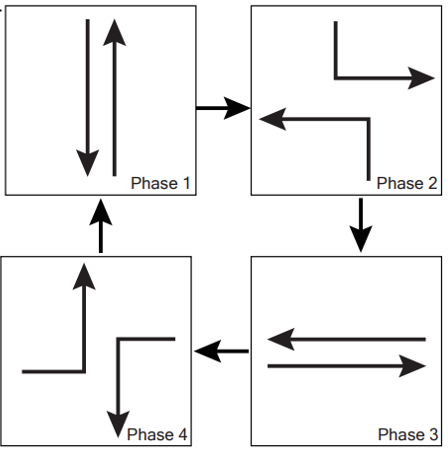
\includegraphics[width=0.3\textwidth]{phases.png}
			\centering
			\caption{The four phases of a traffic light agent considered in \cite{LiDa}. The agent's actions can either maintain the phase or cycle from the current phase to the next}.
			\label{fig:phases}
\end{figure}
		
Another novel approach to represent the state space for a deep reinforcement learning solution is the work presented in \cite{GenRaz16}. First, they partition the traffic lanes into segments of maximum capacity for the discretization of physical space, similar to the idea in \cite{WALRAVEN2016203}. Formally, the state space becomes:
$S \in(\mathbb{B} \times \mathbb{R})^{\frac{1}{c} \times n} \times P$,
where: $l$ is the length of a lane, $c$ is the length of a cell into which the cells have spatially partitioned the space under consideration, $n$ is the size of the physical space (a grid); $\mathbb{B}$ is a boolean value indicating whether or not there is a car at that location, $R$ is the average speed of the cars in that cell, and $P$ is the phase under consideration at that time. If we consider $A$ as the set of actions in the system (similar to Fig. \ref{fig:phases}), then $P is \in \mathbb{B}^{|A|}$. For training their methods, the authors use A3C \cite{MnBA} for efficient parallelization of the experiments. This is something that we also consider in our work and tools. We strongly believe that high level parallelization of experiments is very important to get better policies in less time when computational resources are available.

In \cite{Wu20}, the authors make the transition to a multi-agent reinforcement learning system where each traffic light intersection is a single agent. They modify a version of the DDPG algorithm where the strategies of the agents are synchronized between each traffic light agent. The paper thus proposes a transition from multi-objective learning (where the reward was a single vector simulating multiple agents) to a true multi-agent system. It is also mentioned that the use of LSTM layers for both the Actor and the Critic stabilizes the results, since the agents generally have only partial access to observations in the environment.

The Deep Q-learning implementation is used in many other works, but recently the implementation in \cite{ault} has gained a lead of up to $19.4\%$ over the other solutions using the same learning method. The novelty of their work is the representation of the convolutional Q-network, which uses features such as queue length, number of approaching vehicles, total speed of approaching vehicles, and total waiting time. These are then aggregated into convolutional layers over the lanes that form the same approaching road. The reward formula used is (minus) the total waiting time at the traffic light. 

In \cite{MPLight}, the authors introduce the concept of pressure to coordinate multiple intersections. Pressure is defined as the difference between the length of queues in the arriving lanes of an intersection and the length of queues in the receiving lane of a downstream intersection. They use the FRAP \cite{zheng2019learning} model and pressure as both a state and a reward for a DQN agent distributed across all intersections.

A novel topology and architecture is FMA2C \cite{chu2019multiagent}, which enables cooperation between signal control agents (one per intersection), called workers, in a hierarchical topology. Neighboring workers are coordinated by a local discounted neighbor reward, discounted neighbor states, and joint actions. Workers are the leaf of a hierarchical network in which the leading agents are trained to optimize traffic flow in their assigned region. The higher-level goals of their leading agent are adopted by the workers coordinated below them.

In the same domain, it is also worth noting how Bolt \cite{BOLT} uses a Markov model to estimate the time it takes to get from an origin to a destination. This uses the collected data (as explained in the previous section) and the standard routing engine OSRM \cite{OSRM} to find the shortest path between two points on the globe.

\section{Framework description} \label{sec:frameworkdesc}

The methods behind our framework are based on Deep Reinforcement Learning. The end user can extend it through functional hooks (documentation is available on the repository address) from different points to achieve different: (a) optimization goals as rewards, (b) observations - what information is available from the city/traffic system and how it can be mapped in a numerical format, (c) the algorithms chosen for training the traffic light agents, (d) the platform solution for parallelizing and distributing the work when a wide range of computational resources is available.

\subsection {Single and Multi Agent RL Support}
Our framework supports both single and multi-agent modes. In single agent mode, a single RL agent is created to control all traffic lights in a given area. In multi-agent mode, there is a single agent per traffic light that acts cooperatively as a zero-sum game as much as possible. Figure \ref{fig:softwarestack} shows the software stack used within our framework for experiments between single and multi-agent modes. In single agent mode, the framework can leverage a number of open source libraries to demonstrate its flexibility, such as TFAgents \cite{TFAgents}, PFRL \cite{PFRL}, OpenAI Baselines \cite{baselines}. To provide a similar abstraction for both modes, we use the PeetingZoo library implementation \cite{terry2020pettingzoo}. This allows the framework to provide common OpenAI Gym interfaces \cite{gym} for both modes, as required by the RL research community. In the case of multi-agent RL mode, the machine learning algorithms also need preprocessing operations such as normalizing the length of actions and observations, since the number of lanes may be different for each traffic light agent (intersection). For these operations, we use the Supersuit \cite{SuperSuit}package, which builds wrappers on top of existing code to perform the required preprocessing operations without changing the user's source code. We felt this was the best option available, as it allowed researchers to bring in their existing RL source code more quickly for experimentation. At the execution management level, we leverage the RLlib library \cite{liang2018rllib}, which contains a set of implemented multi-agent algorithms out of the box and a transparent parallelization execution paradigm, to operate on high-performance computing infrastructures.

\begin{figure}[!h]
	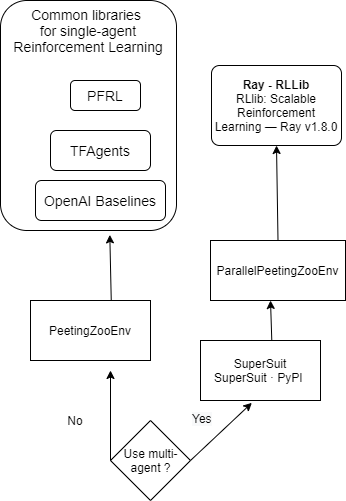
\includegraphics[width=0.35\textwidth]{softwarestack.png}
	\centering
	\caption{The software stack used in our framework to support single and multi-agent reinforcement learning.}
	\label{fig:softwarestack}
\end{figure}

\subsection {Environments Abstraction}
The full structure of a shared environment using the OpenAI Gym \cite{gym} interface is shown in Figure \ref{fig:environmentlayering}. Our environment class is wrapped around two decorators from the PeetingZoo library, which in turn uses some of our preprocessing hooks created with the SuperSuit tool: PadActions and PadObservation - to populate the observation and action spaces so that all agents have the same dimensionality, regardless of the number of lanes each traffic light agent has, OrderEnforcer - to add an order to the execution steps between synchronizing agents (note that we support both asynchronous and synchronous decision making in multi-agent mode; both variants can be addressed in practice, as smart cities can coordinate traffic lights to enforce an order for switching traffic lights), OutOfBoundary - mechanism for checking harmlessness to ensure that data is read/written within correct bounds. The SumoEnvironmentPZ class serves as an adapter between the base environment AECEnv, implemented in the PeetingZoo library based on the Agent Environment Cycle Game \cite{terry2021agent} idea, and the SumoEnvironment class. The difference between PeetingZooEnv and ParallelPeetingZooEnv is that the former assumes that each agent knows what decision the other agents have made at each step, and therefore acts in a fixed order. The second uses the concept of Partially Observable Stochastic Games (POSGs) \cite{DBLP:conf/ijcai/TomasekHABC21}, where the agent cannot see what other agents have done in the current step, i.e. they act in parallel. 

\begin{figure}[!h]
	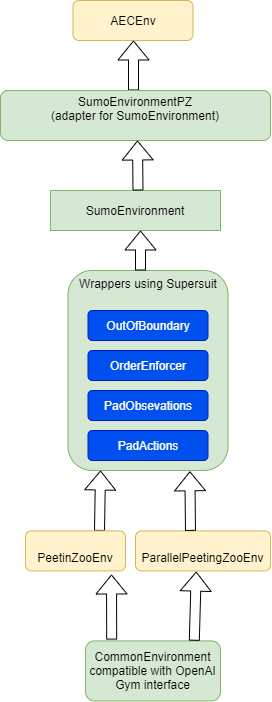
\includegraphics[width=0.35\textwidth]{environmentlayering.png}
	\centering
	\caption{The layered architecture of our OpenAI Gym compatible interface \cite{gym} for environments abstracting both single and multi-agent execution modes. The green colored boxes are implemented in our framework, the yellow ones are from the PeetingZoo library \cite{terry2020pettingzoo}, while the blue color represents reusable components from Supersuit \cite{SuperSuit}}
	\label{fig:environmentlayering}
\end{figure}

Our core implementation of the environment class resides in the SumoEnvironment class, which communicates with SUMO \cite{SUMMO} to manage the simulation. The full picture of this component is shown in Figure \ref{fig:sumoenvironment}. First, a scenario is procedurally loaded into the episode within the SUMO simulator. The scenario contains a traffic infrastructure layout, which can be a real or a toy example for experimentation, and the simulation data for the trajectories of each vehicle, which comes either from recorded real data sets or from fitted probability distributions from which samples are drawn. The second step is to use the API provided by SUMO to retrieve the information about the traffic light phases, the current fixed times and the lane topology at the intersection. For each intersection, the SumoEnvironment instance creates a TrafficLight object instance that contains this information and manages it over time. There are three important operations that can be overridden by the user for their own experiments. We provide state-of-the-art out-of-the-box implementations for each:
\begin{enumerate}
	\item compute\_observation: this function retrieves stored information about the state of each lane at the intersection, current phase, timing information, etc. from SUMO environment. The user can override this to create convolution spaces, for example. We also implement some of the latest proven standard implementations as examples.
	\item compute\_rewards: it returns the reward between different time steps of an episode. The example rewards implemented by default are based on stored data for features such as: average wait time at each traffic light and lane, pressure, total number of vehicles waiting in each lane, and density. The user can calculate other rewards based on these characteristics or expand the possible characteristics according to the documentation.
	\item take\_action: In our default implementation, this follows the state of the art - either no action is taken or it moves to the next phase defined in the simulation data for the particular controlled intersection. A possible example of a custom experiment could be to override the default behavior to switch to different phases as needed, not necessarily in a consecutive cycle as the default.
\end{enumerate}

\begin{figure*}[!h]
	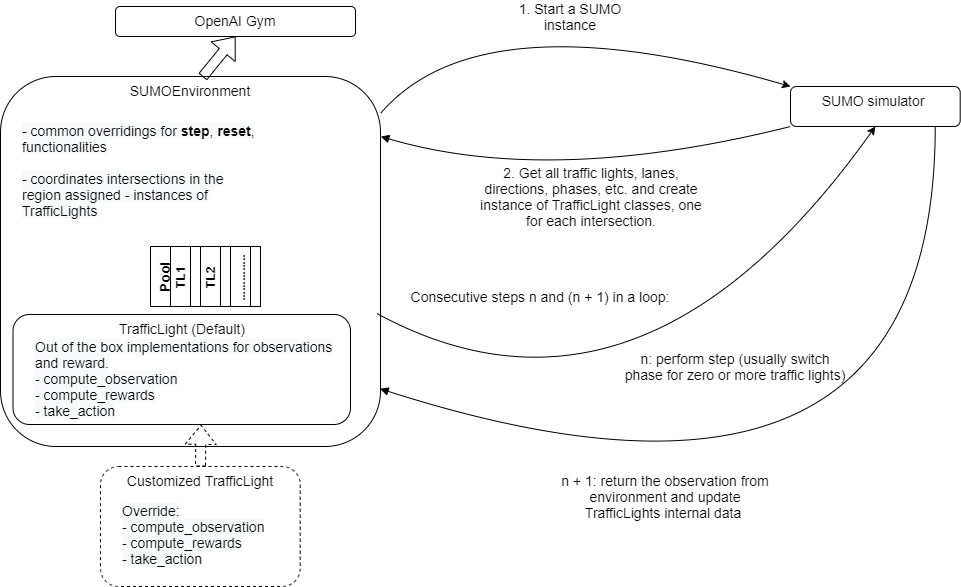
\includegraphics[width=0.99\textwidth]{sumoenvironment.png}
	\centering
	\caption{The interaction flow between an environment class, the SumoEnvironment class, and the simulator SUMO \cite{SUMMO}. The class instantiates a TrafficLight object for each intersection in the scenario loaded in SUMO }.
	\label{fig:sumoenvironment}
\end{figure*}

\section{Evaluation} \label{sec:evaluation}
We evaluated our implementation with the RESCO \cite{ault2021reinforcement} benchmark and show the results in a specific case involving a scenario with 8 intersections in the Cologne (Germany) area (Figure \ref{fig:cologne8}) with real data on road routing, arrival and destination times of cars. As in the original benchmark, we consider the recorded data in the time interval between 25200 and 28800 seconds. The platform used for the training was a cluster of 8 GPUs, Nvidia A100.

\begin{figure}[!h]
	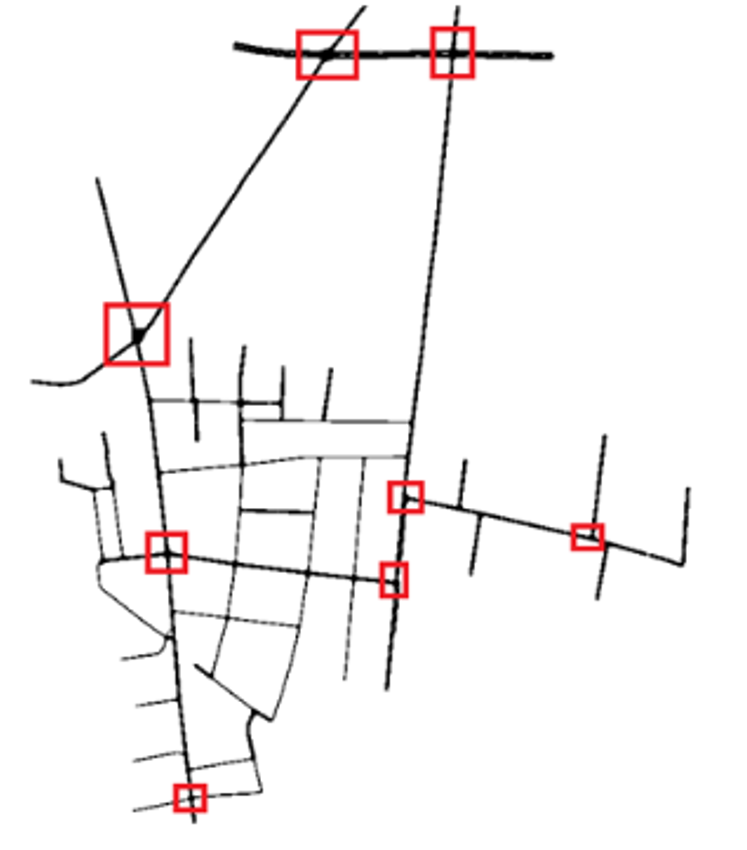
\includegraphics[width=0.25\textwidth]{cologne8.png}
	\centering
	\caption{The region in Cologne where the data used in the analysis was collected. The red boxes show the locations of the intersections. Each is assigned a traffic light agent}
	\label{fig:cologne8}
\end{figure}

Our goal in the evaluation (given also the limited space) was to compare how different RL methods perform from different angles. We chose one of our standard reward, observation, and action spaces by following the literature and observing the similarities between the state of the art \cite{LiDa}. The performance of the algorithms could change significantly if these standard operations are overridden by the user in various ways. The framework provided has a custom plotting mechanism on Tensorboard that is specific to the metrics for the traffic light control optimization problem. According to the documentation provided in the repository, the set of metrics captured can be easily extended by the end user.

The algorithms selected for comparison were chosen from the best performing algorithms in different classes: DQN \cite{DQN} (version with duel networks, target networks and prioritized experience rendering), PPO \cite{schulman2017proximal}, A3C \cite{MnBA} and SAC \cite{ SAC }. We divide the evaluation options into three categories:

\begin{itemize}
	\item Best runs for each algorithm: the graphs in Figures \ref{fig:ev_bestAvgStopped}, \ref{fig:ev_bestMaxStopped}, \ref{fig:ev_bestAvgTime}, \ref{fig:ev_bestMaxTime} below show the best runs for each algorithm evaluated and the following metrics collected: The average and the maximum waiting time of vehicles at a traffic light, the average and the maximum number of vehicles per lane in the evaluated scenario.
	\item Training progress over time: the graphs in Figures \ref{fig:ev_progressAvgStopped}, \ref{fig:ev_progressMaxStopped}, \ref{fig:ev_progressAvgTime}, \ref{fig:ev_progressMaxTime} show how the same set of metrics as in the first point above evolve over time (realtive to the episode index).
	\item Training efficiency: how quickly each algorithm manages to train a given number of episodes (Figure \ref{fig:ev_trainingTime}). This can be valuable for large scenarios (in terms of the number of intersections to optimize). 
\end{itemize}


\begin{figure}[!h]
	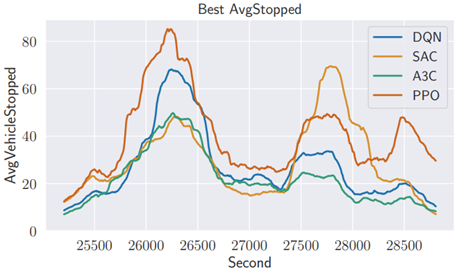
\includegraphics[width=0.25\textwidth]{ev_bestAvgStopped.png}
	\centering
	\caption{Best run comparison for the average number of vehicles stopped at a traffic light}
	\label{fig:ev_bestAvgStopped}
\end{figure}

\begin{figure}[!h]
	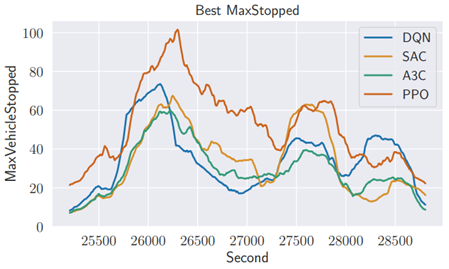
\includegraphics[width=0.25\textwidth]{ev_bestMaxStopped.png}
	\centering
	\caption{Best run comparison for the maximum number of vehicles stopped at a traffic light}
	\label{fig:ev_bestMaxStopped}
\end{figure}

\begin{figure}[!h]
	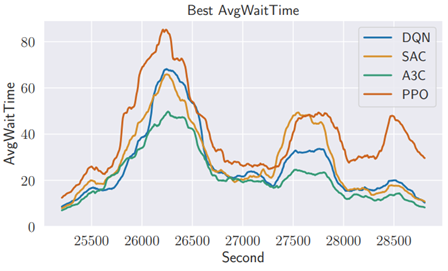
\includegraphics[width=0.25\textwidth]{ev_bestAvgTime.png}
	\centering
	\caption{Best run comparison for the average waiting time of vehicles at a traffic light}.
	\label{fig:ev_bestAvgTime}
\end{figure}

\begin{figure}[!h]
	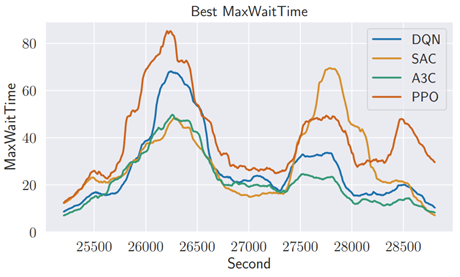
\includegraphics[width=0.25\textwidth]{ev_bestMaxTime.png}
	\centering
	\caption{Best run comparison for the maximum waiting time of vehicles at a traffic light}.
	\label{fig:ev_bestMaxTime}
\end{figure}

%%%%%%%%%%%%%%%%%%%%%%%%%%%%%%%%%%%%%%%%%%%%%%%%%%%%%%%%%%%%%%%%%%%%%
\begin{figure}[!h]
	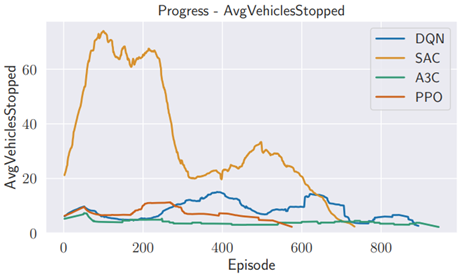
\includegraphics[width=0.25\textwidth]{ev_progressAvgStopped.png}
	\centering
	\caption{Comparison of progress for the average number of vehicles stopped at a traffic light.}
	\label{fig:ev_progressAvgStopped}
\end{figure}

\begin{figure}[!h]
	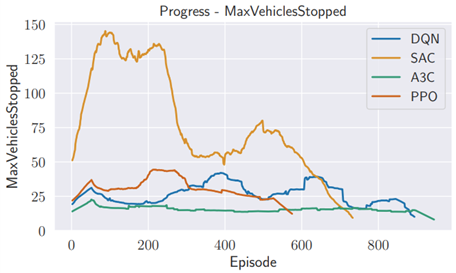
\includegraphics[width=0.25\textwidth]{ev_progressMaxStopped.png}
	\centering
	\caption{Progress comparison for the maximum number of vehicles stopped at a traffic light.}
	\label{fig:ev_progressMaxStopped}
\end{figure}

\begin{figure}[!h]
	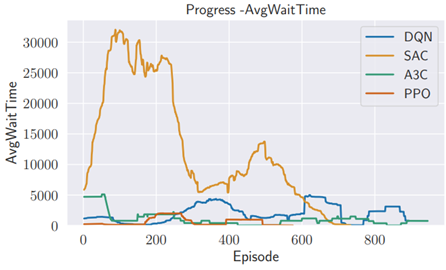
\includegraphics[width=0.25\textwidth]{ev_progressAvgTime.png}
	\centering
	\caption{Progress comparison for the average waiting time of vehicles at a traffic light.}
	\label{fig:ev_progressAvgTime}
\end{figure}

\begin{figure}[!h]
	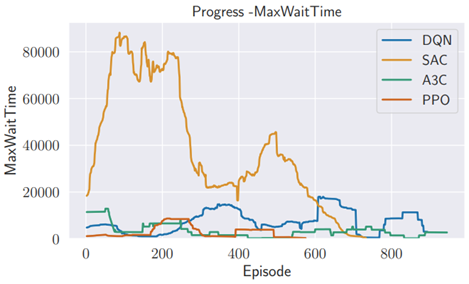
\includegraphics[width=0.25\textwidth]{ev_progressMaxTime.png}
	\centering
	\caption{Progress comparison for the maximum waiting time of vehicles at a traffic light.}
	\label{fig:ev_progressMaxTime}
\end{figure}

%%%%%%%%%%%%%%%%%%%%%%%%%%%%%%%%%%%%%%%%%%%%%%%%%%%%%%%%%%%%%%%%%%%%%

\begin{figure}[!h]
	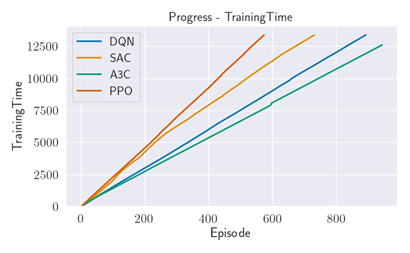
\includegraphics[width=0.35\textwidth]{ev_trainingTime.png}
	\centering
	\caption{Compare training time speed to get to different episode counts.}
	\label{fig:ev_trainingTime}
\end{figure}

As a conclusion from the comparison of algorithms, we can say that the best performance in terms of collected relevant metrics are \cite{MnBA} and \cite{SAC}. When evaluating the most efficient method in terms of training time, PPO \cite{schulman2017proximal} proved to be the optimal solution. This was to be expected considering the theoretical trade-offs between the different classes of algorithms in terms of episode sample complexity and training stability. Future work may draw further conclusions between these classes in the presence of very large scenarios with a significant number of intersections that are simultaneously optimized cooperatively.

\section{\uppercase{Conclusions and future work}}
\label{sec:conclusion}
In this paper, we first presented the state of the art in traffic light control optimization using reinforcement learning methods and dynamic switching of traffic light phases. We then justified the importance of developing a set of tools to separate reinforcement learning (RL) methods from the technical aspects of applying the techniques to the targeted optimization problem. We hope that our work will help the community to perform more experiments in a simpler way than before. In the paper, we have compared a number of well-known algorithms in the field of RL. Our plan is to conduct more experiments and adopt various modern methods from the computer vision field for state mapping. We also want to provide more out of the boxes implementations for various rewards, observations mapping and metrics that prove to outperform the state of the art results. Graph neural networks (GNN) \cite{deepmindblog} that could map the environment states for the RL agents is another topic that interests our group too.


\bibliographystyle{apalike}
{\small
\bibliography{example}}

\iffalse
\section*{\uppercase{Appendix}}

If any, the appendix should appear directly after the
references without numbering, and not on a new page. To do so please use the following command:
\textit{$\backslash$section*\{APPENDIX\}}
\fi

\end{document}

